\section{Rocket-API Service}
\label{sec:komponenten:rocket-api-service}
Um Endnutzern nicht die Last zur Verwaltung von Kubernetes Objekten aufzulegen, dient der Rocket-API Service als Mittelschicht zwischen
Client und Kubernetes. Hierbei wurde mit Hilfe von Googles gRPC\footnote{\href{https://grpc.io/}{gRPC}} Framework
eine API konzipiert, welche Standard CRUD\footnote{Create, Read, Update, Delete} Operationen, sowie das Auslesen
von Containerlogs implementiert.
Jeder Client nutzt das OpenID Connect Protokoll, um den Nutzer an der Authentifizierungsstelle, dem Keycloak
Server, anzumelden. Sobald der Client das erhaltene OpenID Token von Keycloak zurück bekommt,
wird es als HTTP Header in jeder Anfrage an den Rocket API-Service mitgeliefert.
Dargestellt ist der beschriebene Ablauf in Abbildung \ref{fig:rocket-api-service-flow}.
Um sicherzustellen, dass jeder Nutzer nur auf seine eigenen Services zugreifen kann, 
werden alle Anfragen an die Kubernetes API mithilfe des beigelieferten Tokens gestellt.

\begin{figure}[]
  \centering
  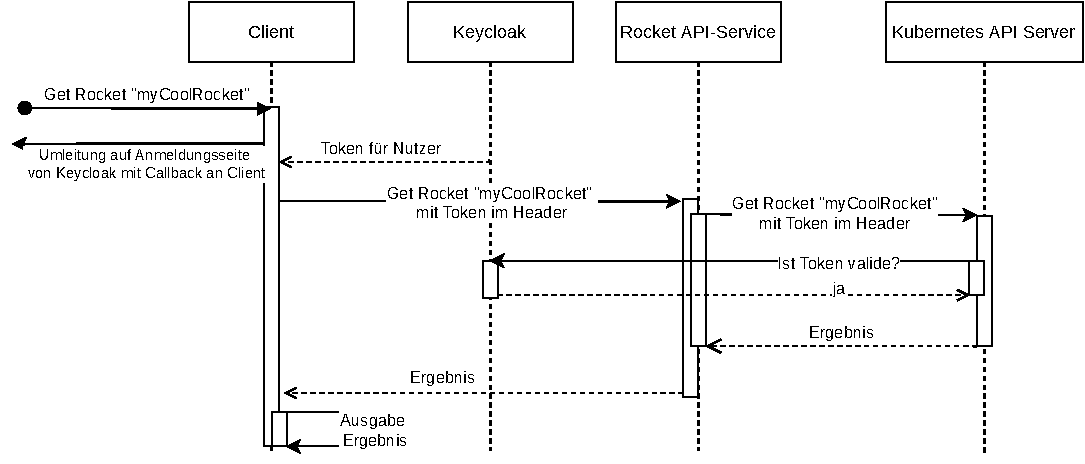
\includegraphics[height=0.5\textwidth]{gfx/chapters/3_komponenten/api-service-flow.pdf}
  \caption{Ablauf des Rocket API-Services}
  \label{fig:rocket-api-service-flow}
\end{figure}

Durch das Auslagern von CRUD Operationen und Tenant Operationen in
verschiedene Services, kann eine unabhängige Entwicklung der beiden Services stattfinden.